\documentclass[10pt]{beamer}

% --- Packages de base ---
\usepackage[utf8]{inputenc}
\usepackage[T1]{fontenc}
\usepackage[french]{babel}
\usepackage{booktabs}
\usepackage{amsmath}
\usepackage{amsfonts}
\usepackage{amssymb}
\usepackage{graphicx}
\usepackage{hyperref}
\usepackage{csquotes}
\usepackage{booktabs}
\usepackage{multirow}

% Thème et Personnalisation Visuelle
\usetheme{Madrid}
\usecolortheme{whale}

% Définition d'une palette de couleurs (couleur LAAS)
\definecolor{laasblue}{RGB}{12, 35, 64}
\definecolor{laasaccent}{RGB}{0, 150, 136}
\definecolor{bglight}{RGB}{248, 249, 250}

% Application des couleurs au thème Beamer
\setbeamercolor{palette primary}{bg=laasblue, fg=white}
\setbeamercolor{palette secondary}{bg=laasblue!85, fg=white}
\setbeamercolor{palette tertiary}{bg=laasblue!70, fg=white}
\setbeamercolor{titlelike}{parent=palette primary}
\setbeamercolor{structure}{fg=laasblue}

% Personnalisation esthétique des blocs
\setbeamercolor{block title}{bg=laasblue!90, fg=white}
\setbeamercolor{block body}{bg=bglight, fg=black}
\setbeamercolor{block title alert}{bg=red!80!black, fg=white}
\setbeamercolor{block body alert}{bg=red!5, fg=black}
\setbeamercolor{block title example}{bg=laasaccent, fg=white}
\setbeamercolor{block body example}{bg=laasaccent!5, fg=black}

% Paramétrages généraux
\setbeamertemplate{navigation symbols}{}
\setbeamertemplate{footline}[frame number]
\setbeamertemplate{caption}[numbered]
\setbeamerfont{footnote}{size=\scriptsize}

\usepackage[backend=bibtex, style=numeric]{biblatex}
\addbibresource{biblio.bib}

% Diapo titre
\title[Avancée des Recherches]{Amélioration de Méthodes de Benders pour un
problème de planification robuste sous incertitude}
\subtitle{Soutenance}

\author[M. Francine-Habas]{
    Mathis Francine-Habas\inst{1, 2} \and 
    Christian Artigues\inst{1} \and 
    Romain Guillaume\inst{2}
}

\institute[UT3 - LAAS]{
    \inst{1} LAAS-CNRS, ENAC, Université de Toulouse, France\\
    \vspace{0.2cm}
    \inst{2} IRIT-CNRS, HEROIC-ANITI, Université Jean-Jaurès, France
}

\date{\today}

\titlegraphic{
\includegraphics[height=1.2cm]{images/inst3.png}
\hspace{1cm} 
\includegraphics[height=1.2cm]{images/inst4.png}}

\logo{
\includegraphics[height=0.6cm]{images/inst3.png}}

\begin{document}

\begin{frame}[plain]
    \titlepage
\end{frame}

\begin{frame}{Plan de la présentation}
    \tableofcontents[hideallsubsections]
\end{frame}

\section{Présentation du Sujet}

\begin{frame}{Présentation du Sujet}{Contexte industriel \& Problème}
    \begin{block}{Contexte de la Recherche}
        \begin{itemize}
        	\item \textbf{Cadre :} Chaire HEROIC\footnote{Hybridizing Learning, seaRch and combinatorial Optimization for Industrial deCision-making} ANITI appliqué aux chaînes logistiques d'AIRBUS.
        	\item \textbf{Problème central :} Dimensionnement de lots avec capacités : \textit{minimiser} les coûts ; \textit{maximiser} les bénéfices.
        	\item \textbf{Objectif :} Produire ce plan de production tout en respectant les capacités industrielles.
            \item Suite des travaux de recherche de Tom Portoleau (2022)\footfullcite{these-portoleau}.
        \end{itemize}
    \end{block}

    \begin{alertblock}{Problématique}
        Comment optimiser la planification robuste sous incertitude, en milieu industriel, grâce à la méthode de Benders ?
    \end{alertblock}
\end{frame}

\begin{frame}{Présentation du Sujet}{Le Lot-Sizing}
    \begin{block}{Le Lot-Sizing Déterministe}
        \begin{itemize}
            \item \textbf{Exemple :} Une usine doit fournir des pièces de fuselage.
            \item Allumer la chaîne de production coûte cher (\textit{Setup cost}).
            \item Stocker les pièces en avance coûte cher (\textit{Holding cost}).
            \item \textbf{Solution :} On groupe les productions en "lots" calculés à l'avance pour équilibrer ces coûts, \textcolor{red}{en supposant que la demande est parfaitement connue}.
        \end{itemize}
    \end{block}

    \begin{alertblock}{La réalité : L'Incertitude}
        \begin{itemize}
            \item En réalité, un client peut décaler sa commande.
            \item Si le plan de production est trop rigide, on s'expose à des pénalités de rupture (\textit{Backorder cost}). Il faut un plan \textbf{robuste}.
        \end{itemize}
    \end{alertblock}
\end{frame}

\begin{frame}{Présentation du Sujet}{Modélisation de l'incertitude}
	\begin{block}{L'approche $MinMax$}
		\begin{itemize}
			\item \textbf{Le défi :} La demande client est soumise à de fortes incertitudes.
			\item \textbf{Notre modélisation :} Incertitude portant sur la demande cumulée, régie par un budget d'incertitude ($\Gamma$) (voir \ref{fig:incert_periode_demande}).
			%\item \textbf{Avantage industriel :} Permet de modéliser le report de demande de façon plus réaliste qu'une incertitude période par période.
			\item \textbf{Approche $MinMax$ :} "Trouver le plan le moins coûteux face au pire des scénarios possibles".
		\end{itemize}
	\end{block}
\end{frame}

\begin{frame}{Concept de l'algorithme de Benders Adverse}{Défence/Attaque}
    \begin{columns}[c]
        % Colonne Texte
        \begin{column}{0.5\textwidth}
            \small
            \begin{block}{Le Maître (La Défense)}
                \begin{itemize}
                    \item Fixe un plan de production initial.
                    \item \textbf{But :} Minimiser les coûts.
                \end{itemize}
            \end{block}
            
            \begin{block}{Le Sous-problème (L'Attaque)}
                \begin{itemize}
                    \item Observe le plan du Maître.
                    \item \textbf{But :} Explorer toutes les possibilités d'incertitude pour trouver le scénario qui coûtera le plus cher.
                \end{itemize}
            \end{block}

            \begin{alertblock}{Boucle d'arrêt}
                $\textit{IF}\, obj_{value}\text{(Maître)} == obj_{value}\text{(Adv)}\, \textit{THEN}
                
                \hookrightarrow\,\text{plus de dégradation possible}$.
            \end{alertblock}
        \end{column}
        
        \begin{column}{0.5\textwidth}
            \begin{figure}[H]
                \centering
                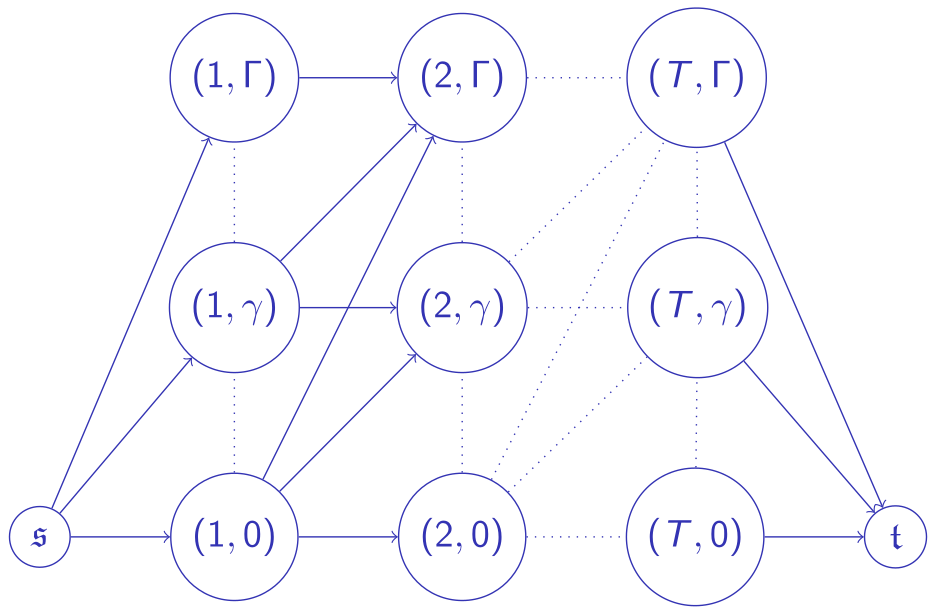
\includegraphics[width=\linewidth]{images/budget_graph.png} 
                \caption{Graphe de budget. \cite{these-portoleau}}
            \end{figure}
        \end{column}
    \end{columns}
\end{frame}

\section{L'Algorithme de Benders Adverse et sa Variante}

\begin{frame}[shrink=1]{Concept de l'algorithme de Benders Adverse}{Méthode de Benders Adverse (Étendu)}
    
    \begin{columns}[T] 
        \begin{column}{0.5\textwidth}
        
            \vspace{-0.5cm}
            
            \begin{figure}
                \centering
                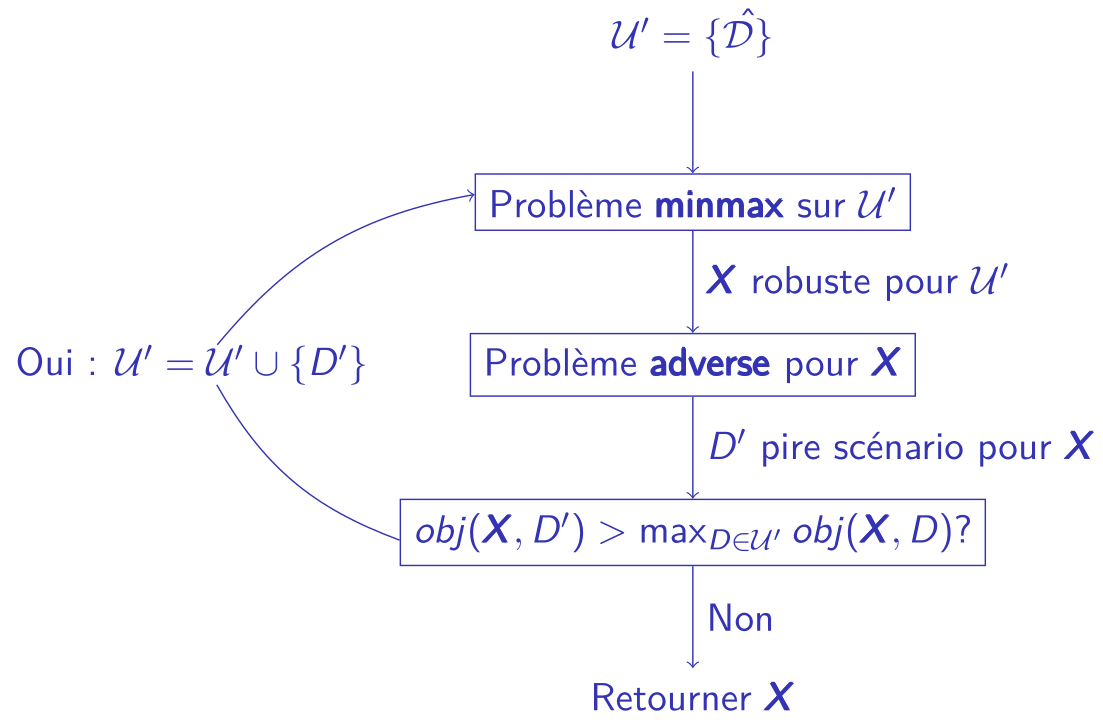
\includegraphics[width=\linewidth]{images/graph_benders_classique.png}
                \caption{Benders Adverse (BA). \cite{portoleau_SMAI}}
                \label{fig:algo_benders_classique}
            \end{figure}
            
            \vspace{-0.5cm}
            
            \begin{itemize}
                %\item \textbf{Problème Maitre :} Calcule le plan de production.
                \item \textbf{Problème adverse :} Identifie l'unique scénario de demande.
            \end{itemize}
        \end{column}
        
        \begin{column}{0.5\textwidth}
            
            \vspace{-0.5cm}
            
            \begin{figure}
                \centering
                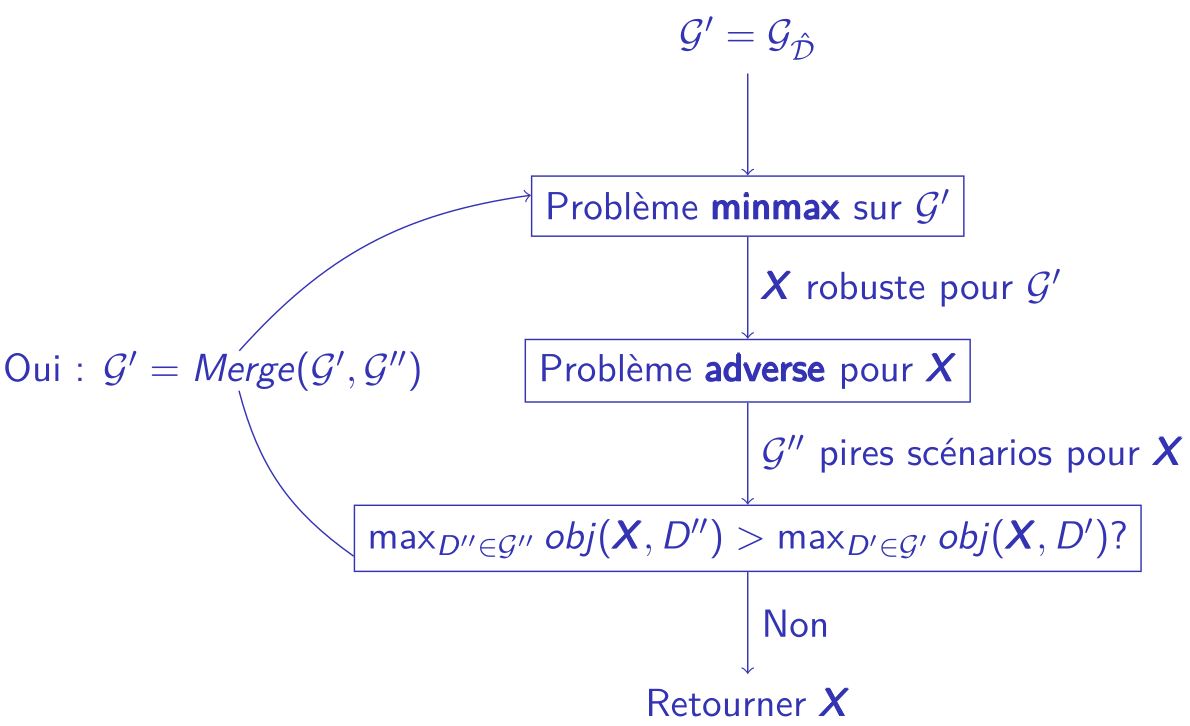
\includegraphics[width=\linewidth]{images/graphe_benders_etendue.png}
                \caption{Benders Adverse Étendu (BAE). \cite{portoleau_SMAI}}
                \label{fig:algo_benders_etendu}
            \end{figure}

            \vspace{-0.6cm}
            
            \begin{itemize}
                \item \textbf{L'innovation :} Retourne un sous-graphe de budget regroupant un ensemble de mauvais scénarios.
                \item \textcolor{red}{\textbf{Idée sous-jacente} : Le Maître apprend plus vite et nécessite moins d'itérations pour converger.}
            \end{itemize}
        \end{column}
    \end{columns}
\end{frame}

\section{Limites et Heuristiques Envisagées}

\begin{frame}{Limites et Heuristiques Envisagées}
	\begin{block}{Limites}
		\begin{itemize}
			\item \textbf{Limite de l'approche $BAE$ :} La sélection basée sur un pourcentage de tolérance peut générer des scénarios très similaires.
			\item \textcolor{red}{\textbf{Mon objectif :} Trouver des heuristiques permettant de maximiser la diversité des scénarios remontés.}
		\end{itemize}
	\end{block}
	
	\begin{block}{Heuristiques}
		\begin{itemize}
			\item \textbf{Principe :} Sélectionner des scénarios "orthogonaux" qui dégradent le plan de production à des périodes différentes.
			\item \textbf{Pistes d'implémentation :} Définition d'une métrique de distance ; Approche gloutonne.
		\end{itemize}
	\end{block}

\end{frame}

\section{Résultats Obtenus Initialement}

\begin{frame}{Résultats Obtenus Initialement}
    \begin{figure}
        \centering
        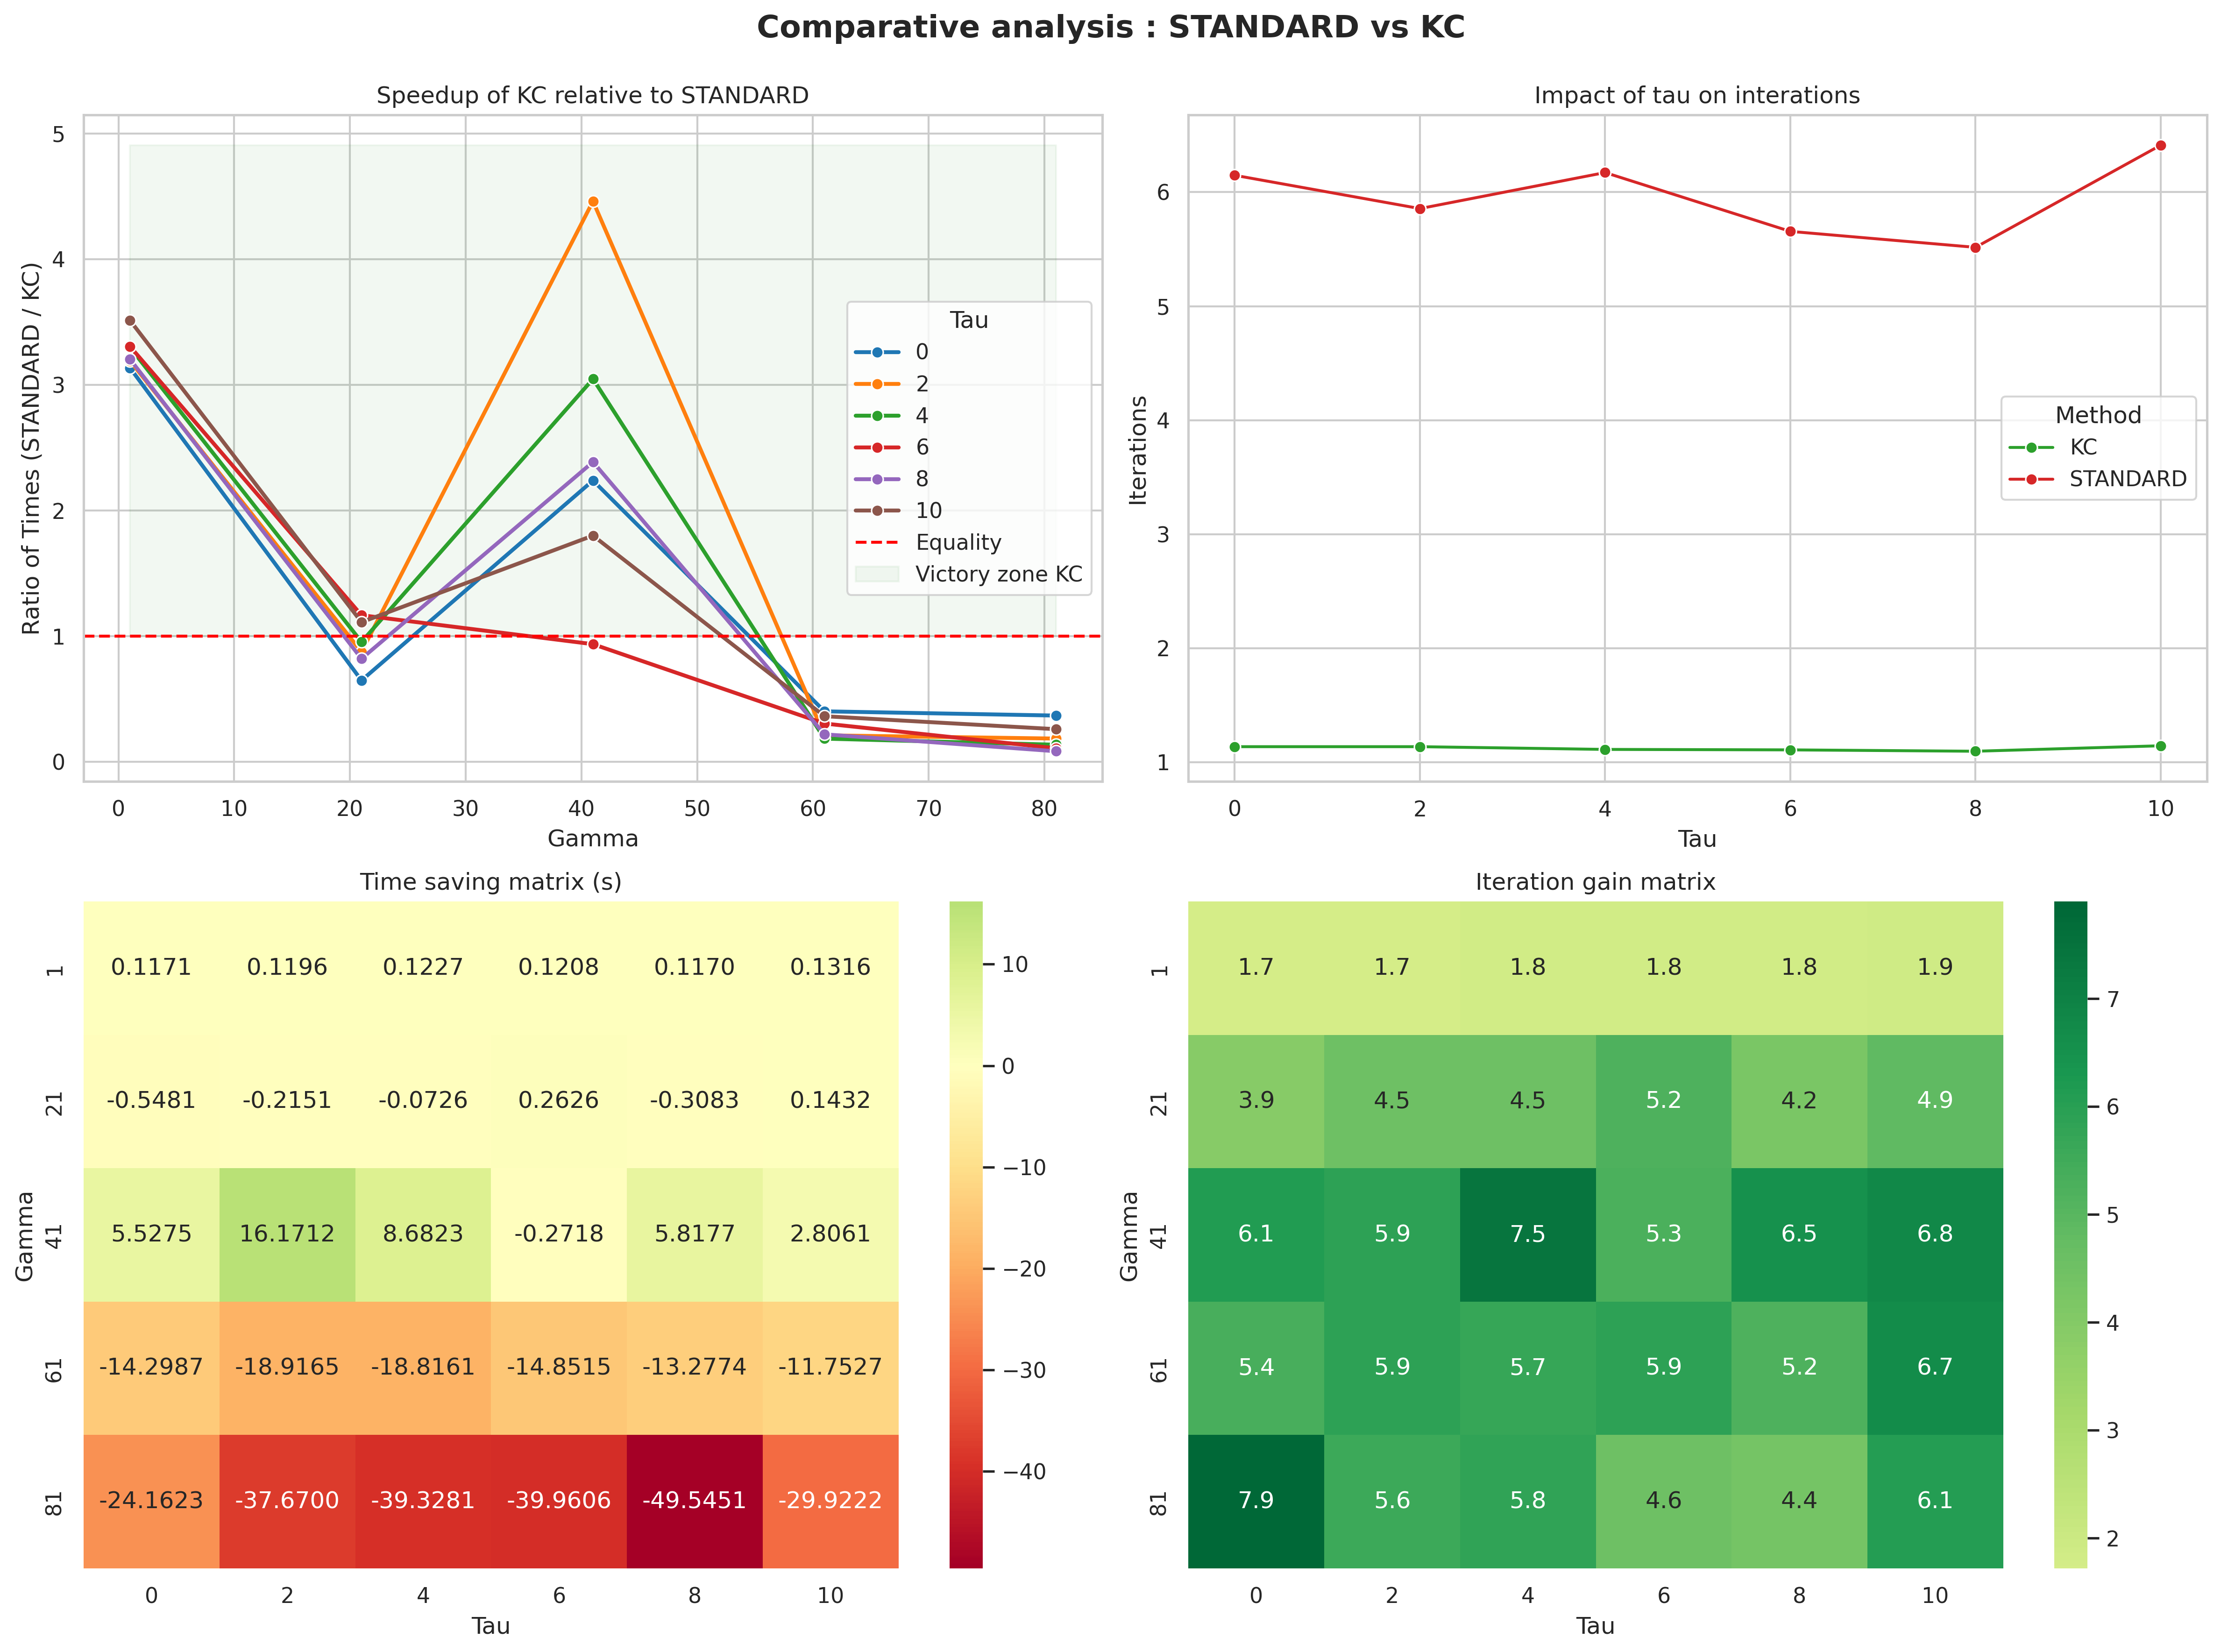
\includegraphics[width=0.8\linewidth]{images/result_benders_2026-06-26_1408_n=15_l=2000_classic_STANDARD_KC.png}
        \caption{$BA\, VS\, BAE_{sans\,heuristique}$.}
        \label{fig:graphe_res}
    \end{figure}    
\end{frame}

\section{Perspectives}

\begin{frame}{Perspectives}{Court et Moyen Terme}
    \begin{block}{Objectifs à Court Terme}
        \begin{itemize}
            \item Modéliser et implémenter de nouvelles heuristiques permettant d'optimiser l'approche $BAE$.
            \item Affiner les coupes combinatoires pour accélérer la convergence.
        \end{itemize}
    \end{block}

    \begin{block}{Objectifs à Moyen Terme}
        \begin{itemize}
            \item Comparer les temps de convergence entre $BA\, VS\, BAE_{classic}$ \& $BAE_{heuristic}$.
            \item Rédaction de l'article.
        \end{itemize}
    \end{block}
\end{frame}

\begin{frame}
    \begin{center}
        \Huge \textcolor{laasblue}{\textbf{Merci pour votre attention !}}
        
        \vspace{1.2cm}
        \Large Avez-vous des questions ?
    \end{center}
\end{frame}

\section*{Bibliographie}

\begin{frame}[allowframebreaks]{Bibliographie}
    \printbibliography
\end{frame}

\section*{Annexes}

\begin{frame}{Annexe 1}
	\centering
	\begin{figure}
		\centering
		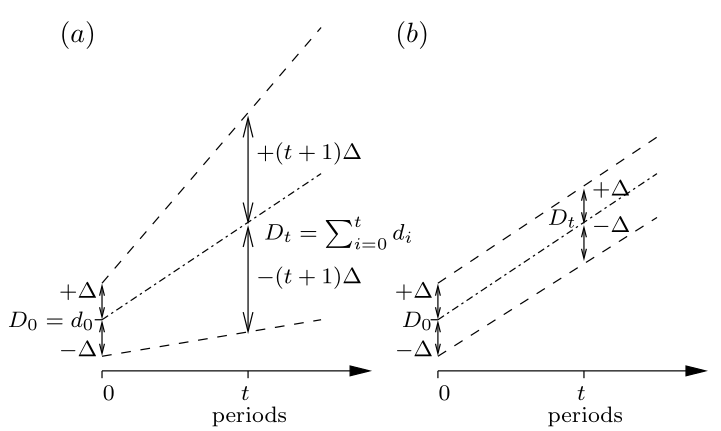
\includegraphics[width=0.6\linewidth]{images/incertitude_periode_demande.png}
		\caption{\textbf{(a)} : Incertitude sur la période ; \textbf{(b)} : Incertitude sur la demande.\cite{portoleau_SMAI}}
		\label{fig:incert_periode_demande}
	\end{figure}
\end{frame}

\begin{frame}[shrink=1]{Annexe 2}
    \subsection{Lot-sizing problem}
    
    \begin{align}
        \min \quad & \sum_{t=1}^{T} \left( c^I I_t + c^B B_t + c^P y_t - b^P s_t \right) \notag \\
        \text{s.t.} \quad & B_t - I_t = D_t - X_t && \forall t \in [T], \\
        & \sum_{i=1}^{t} s_i = D_t - B_t && \forall t \in [T], \\
        & X_t - X_{t-1} \leq M y_t && \forall t \in \{2, \dots, T\}, \\
        & X_1 \leq M y_1, \\
        & B_t, I_t, s_t \geq 0 && \forall t \in [T], \\
        & y_t \in \{0, 1\} && \forall t \in [T], \\
        & x \in \mathbb{X} \subseteq \mathbb{R}^T_+ && \forall t \in [T]
    \end{align}
    
    \begin{itemize}
        \item $D_t = \sum_{i=1}^{t} d_i$ : la demande cumulée jusqu'à la période $t$,
        \item $X_t = \sum_{i=1}^{t} x_i$ : la production cumulée jusqu'à la période $t$,
        \item $\mathbb{X}$ : ensemble des productions possibles représentées par des contraintes linéaires,
        \item $y_t \in \{0, 1\}$ : indicatrice de la production à la période $t$,
        \item $I_t, B_t, s_t$ : le niveau des stocks, des commandes en retard et les ventes du produit à la fin de la période $t \in [T]$.
    \end{itemize}
\end{frame}

\begin{frame}{Annexe 3}
	\begin{theorem}
		Le problème $ADV$ sous l'incertitude $\mathcal{U}$ est \textit{NP-dur} au sens faible (Guillaume, Kasperski, Zielinski, 2022).\cite{GOERIGK2023108941}
	\end{theorem}
\end{frame}

\begin{frame}{Annexe 4}
	\begin{theorem}
		Le problème $ADV$ sous l'incertitude $\mathcal{U}$ peut être résolu en $\mathcal{O}(T\Gamma\Delta_{max})$ temps, où $\Delta_{max}=max_{t\in[T]}$ et $\Delta_{max} \leq\Gamma$ (Guillaume, Kasperski, Zielinski, 2022).\cite{GOERIGK2023108941}
	\end{theorem}
\end{frame}

\begin{frame}{Annexe 5}
	\begin{table}[]
        \centering
        \begin{tabular}{@{}|l|llllll@{}}
        \toprule
        \multirow{2}{*}{$\Gamma$ \textbackslash{} Methode} & \multicolumn{2}{l|}{BA}                                & \multicolumn{2}{l|}{$BAE_{all}$}                              & \multicolumn{2}{l|}{$BAE_{few}$}                              \\ \cmidrule(l){2-7} 
                                                      & iter.                     & time                       & iter.                     & time                       & iter.                     & time                       \\ \midrule
        1                                             & \multicolumn{1}{l|}{3.27} & \multicolumn{1}{l|}{0.63}  & \multicolumn{1}{l|}{\textbf{1.82}} & \multicolumn{1}{l|}{\textbf{0.19}}  & \multicolumn{1}{l|}{\textbf{1.82}} & \multicolumn{1}{l|}{\textbf{0.19}}  \\ \midrule
        20                                            & \multicolumn{1}{l|}{6.18} & \multicolumn{1}{l|}{10.34} & \multicolumn{1}{l|}{\textbf{1.82}} & \multicolumn{1}{l|}{7.82}  & \multicolumn{1}{l|}{3.82} & \multicolumn{1}{l|}{\textbf{1.79}}  \\ \midrule
        40                                            & \multicolumn{1}{l|}{4.81} & \multicolumn{1}{l|}{12.62} & \multicolumn{1}{l|}{\textbf{1.81}} & \multicolumn{1}{l|}{29.36} & \multicolumn{1}{l|}{3.90} & \multicolumn{1}{l|}{\textbf{6.29}}  \\ \midrule
        60                                            & \multicolumn{1}{l|}{6.81} & \multicolumn{1}{l|}{21.18} & \multicolumn{1}{l|}{\textbf{1.90}} & \multicolumn{1}{l|}{62.2}  & \multicolumn{1}{l|}{5.72} & \multicolumn{1}{l|}{\textbf{18.30}} \\ \midrule
        80                                            & \multicolumn{1}{l|}{8.09} & \multicolumn{1}{l|}{42.89} & \multicolumn{1}{l|}{\textbf{1.90}} & \multicolumn{1}{l|}{90.4}  & \multicolumn{1}{l|}{4.09} & \multicolumn{1}{l|}{\textbf{21.14}} \\ \midrule
        100                                           & \multicolumn{1}{l|}{5.81} & \multicolumn{1}{l|}{\textbf{28.45}} & \multicolumn{1}{l|}{\textbf{2.0}}  & \multicolumn{1}{l|}{134}   & \multicolumn{1}{l|}{5.18} & \multicolumn{1}{l|}{44.0}  \\ \bottomrule
        \end{tabular}
        \caption{Nombre d'itérations et temps d'exécution (en secondes) moyen pour chacune des trois méthodes. (Table extraite de \cite{portoleau_SMAI})}
    \end{table}
\end{frame}

\end{document}